\documentclass{standalone}
\usepackage{tikz}
\usepackage{amsmath}
\usetikzlibrary{matrix,chains,positioning,decorations.pathreplacing,arrows}
\usetikzlibrary{positioning, calc, chains, automata}
\usetikzlibrary{decorations.pathreplacing}
\begin{document}


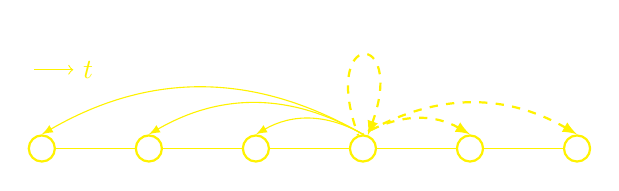
\begin{tikzpicture}[draw=yellow, item/.style={circle,draw,thick,align=center},
itemc/.style={item,on chain,join}]

%encoder
\begin{scope}[start chain=going right,nodes=itemc,every
join/.style={},local bounding box=chain, xshift=-7cm]
\path 
	node[color=yellow] (e1) {} 
	node[color=yellow] (e2) {} 
	node[color=yellow] (e3) {} 
	node[color=yellow] (e4) {} 
	node[color=yellow] (e5) {} 
	node[color=yellow] (e6) {}; 
\end{scope}

\draw[->, color=yellow] (-7.1, 1) --  ++(.5, 0) node[right] {$t$} ;

\foreach \T in {1,2,3} 
{\path[latex-] (e\T.north) edge[bend left=30] (e4.north); }

\foreach \T in {5,6} 
{\path[thick, dashed, latex-] (e\T.north) edge[bend right=30] (e4.north); }


\path[thick, dashed, latex-] (e4) edge[loop above, out=70, in=110, looseness=30] (e4);
\end{tikzpicture}



\end{document}